To determine whether our \textbf{multi-modal} approach outperformed a traditional \textbf{vision only} approach to the language grounding problem in our \ispy task, we measured the average number of robot guesses and human guesses in games played with each fold of objects.
Note that the systems were identical in fold 0 since both are completely untrained.
When \ispy had been played with all folds, we trained the systems on all available data to calculate predicate classifer agreement metrics with human labels.

\begin{figure}
\centering
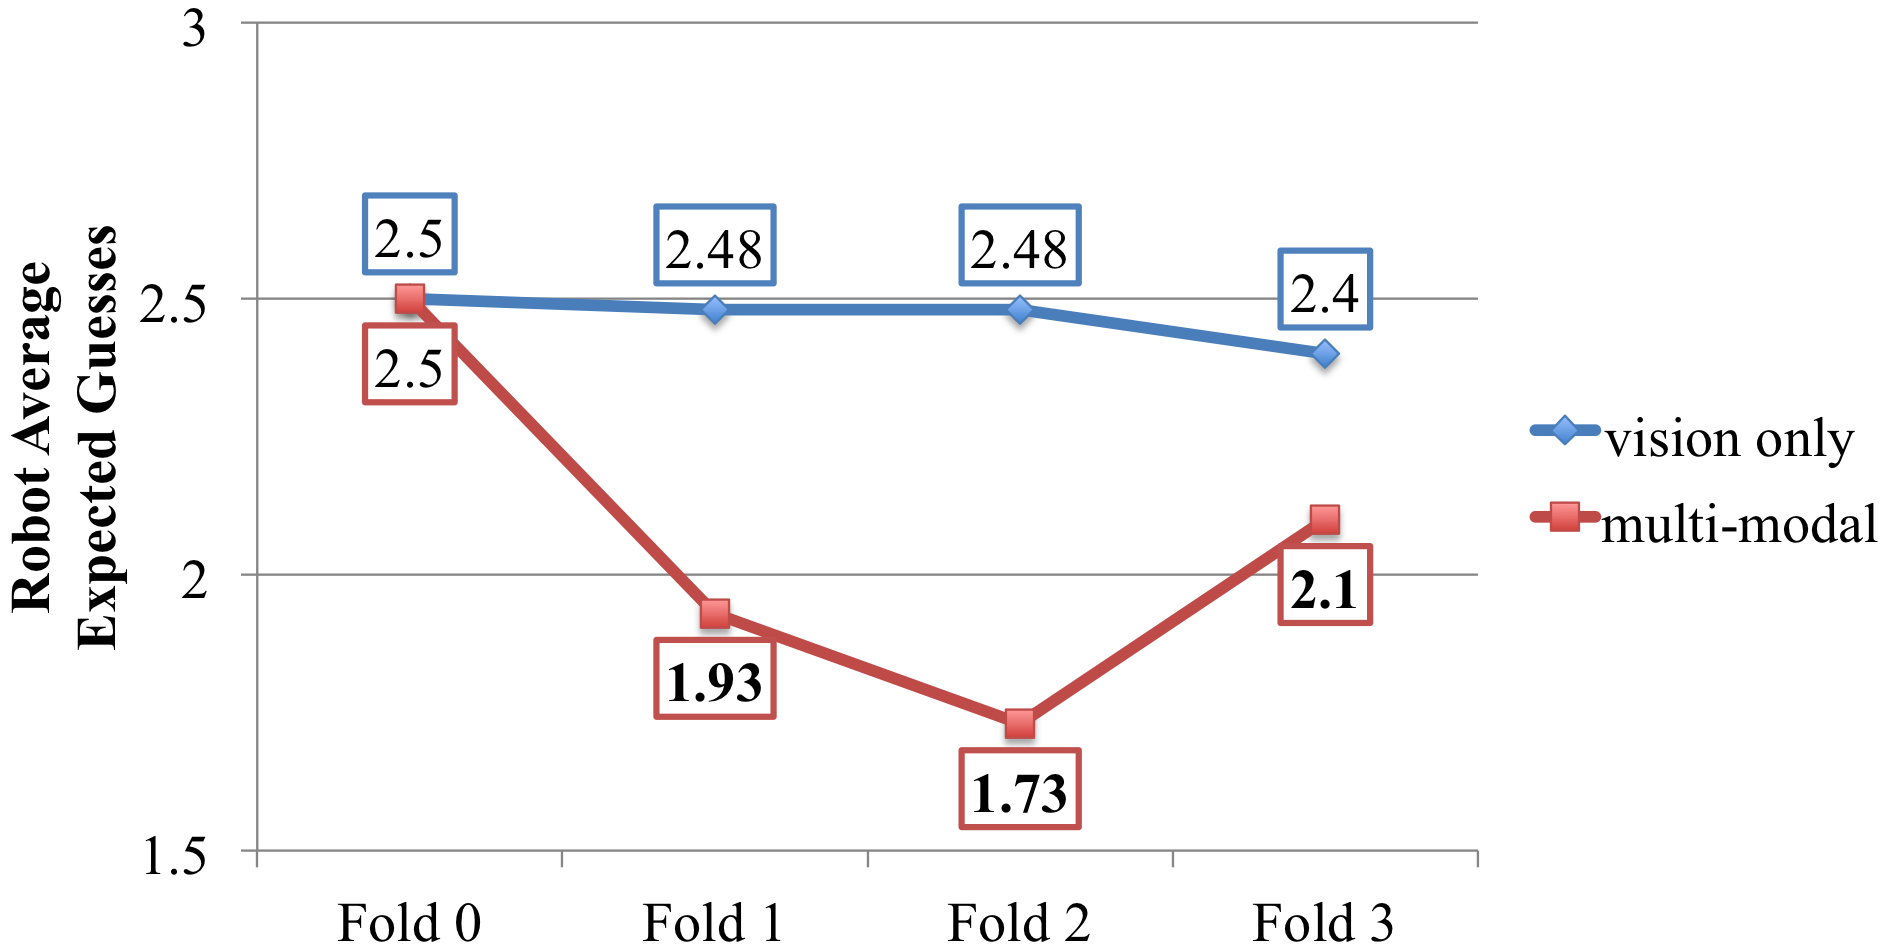
\includegraphics[width=0.5\textwidth]{figures/robot_guesses.png}
\caption{Average expected number of guesses the robot made on each human turn. Numbers in \textbf{bold} are significantly lower than the average at fold 0 with $p<0.05$ (unpaired Student's $t$-test)}
\label{fig:robot_guesses}
\end{figure}

\paragraph{Robot guess.}
Figure~\ref{fig:robot_guesses} shows the average number of robot guesses for the games in each fold. Because we had access to the order in which the robot intended to guess each object along with which objects were tied, we calculated the {\it expected} number of robot guesses for each turn.
For example, if all four objects were tied for first, the number of guesses for that turn was deemed to be 2.5, regardless of whether it got (un)lucky and picked the correct object (last)first.
\footnote{2.5 is the expected number for 4 tied objects because the probability of picking in any order is equal, so the average turn `score' is $\frac{1+2+3+4}{4} = \frac{10}{4} = 2.5$}.

After training on just one fold, our \textbf{multi-modal} approach performs statistically significantly better than the expected number of turns for guessing (the only strategy for the untrained fold 0 system) for the remainder of the games.
The \textbf{vision only} system, by contrast, is never able to differentiate itself from random guessing, even as more training data becomes available.
Additionally, on folds 1 and 2, a paired Student's $t$-test reveals that the \textbf{multi-modal} system outperms the \textbf{vision only} system on a subject-by-subject basis ($p<0.05$).

\paragraph{Human guess.}
Since we have no such intuition into a human's guess order, we simply counted how many times a subject picked a new object as a guess.
We discarded guesses on the same object twice in a row, as these were often just double detections from the robot, but we counted guesses on the same object with an intervening guess after observing some users insisting to the robot that the object they had chosen before was correct.

Neither the \textbf{vision only} nor \textbf{multi-modal} system's performance improves on this task with statistical significance as more training data is seen.
In fact, human guesses hovered around 2.5 (random guessing) per robot turn throughout all levels of training and sets of objects.
The study coordinator who remained in the room during all trials noted that subjects tended to resort to guessing (just passing to the next closest object and trying them all this way) after not getting the correct object on their first try.

This result highlights the difficulty of the robot's turn in an \ispy framework, which requires not just good coverage of grounded words (as when figuring out what object the human is describing), but also high accuracy when using classifiers on new objects.
Many context classifiers which had few examples could achieve confidence $kappa=1$ (see Section~\ref{ssec:mmp}, making the predicates they represented more likely to be chosen to describe objects.
It is possible that the system would have performed better on this metric if the predicate scoring function $R$ additionally favored predicates for which many labels had been gathered over sparsely labeled predicates which could carry deceptively high context $kappa$ values.

\paragraph{Predicates.}
We analyzed the predicate classifiers built by the \textbf{vision only} and \textbf{multi-modal} systems.
After training the predicate classifiers using data gathered over all folds of objects, we calculated the precision, recall, $F_1$, and $\kappa$ scores of each against the gold human labels on which they were trained.
Table~\ref{tab:predicate_results} gives these metrics for the 54 predicates shared between the systems.

\begin{table}
\centering
\begin{tabular}[h]{|l|r|r|}
	\hline
	\bf Metric & \multicolumn{2}{c|}{\bf System} \\ \hline \hline
	& \bf vision only & \bf multi-modal \\ \hline
	precision & .306 & .497\textbf{*} \\
	recall & .340 & .530\textbf{*} \\
	\bf $F_1$ & .317 & .498\textbf{*} \\
	\bf $\kappa$ & .105 & .212\textbf{*} \\ \hline
\end{tabular}
\caption{Agreement metrics of predicate classifiers shared between the \textbf{vision only} and \textbf{multi-modal} systems.
\textbf{*} indicates a statistically significantly greater value with $p<0.05$ (Student's paired $t$-test).}
\label{tab:predicate_results}
\end{table}

There were 129 predicates total between both systems.
The \textbf{multi-modal} system outperforms the \textbf{vision only} system with the same statistical significance presented in Table~\ref{tab:predicate_results} when performing an unsigned $t$-test across all 129 predicates as well, with the exception of $\kappa$ differing with $p<0.1$, rather than $p<0.05$.

Then across the objects our robot explored, our \textbf{multi-modal} system achieves consistently better agreement with human assignments of predicates to objects than does the \textbf{vision only} system.